\section{Examples}
\subsection{A simple case}

\begin{figure}[!htb]
\centering
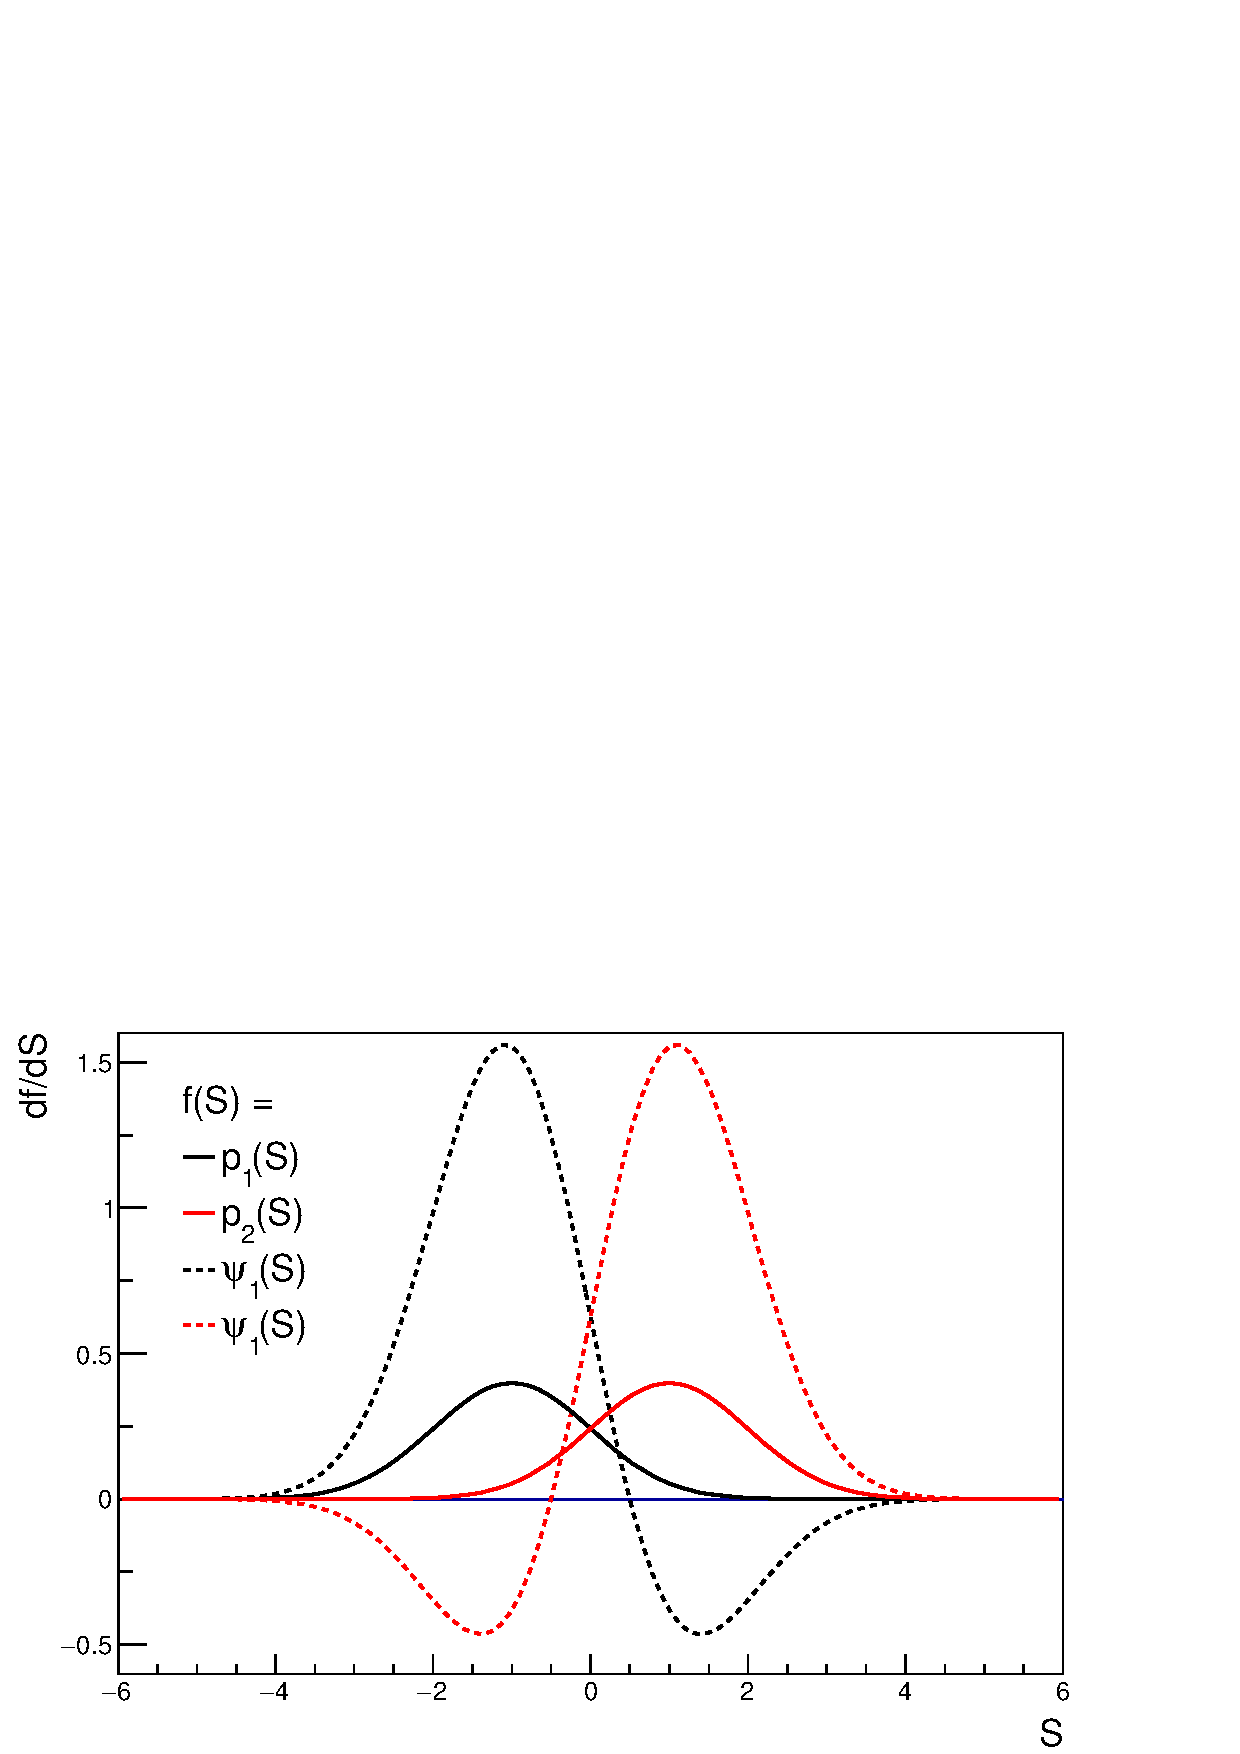
\includegraphics[width=0.7\textwidth]{../png/figGaus2.png}
\caption{Two Gaussian detector responses ($\Delta_{12} = 2$) and relative
  $\psi(S)$ amplitudes.}
\label{fig:Gaus2}
\end{figure}

\begin{figure}[!htb]
\centering
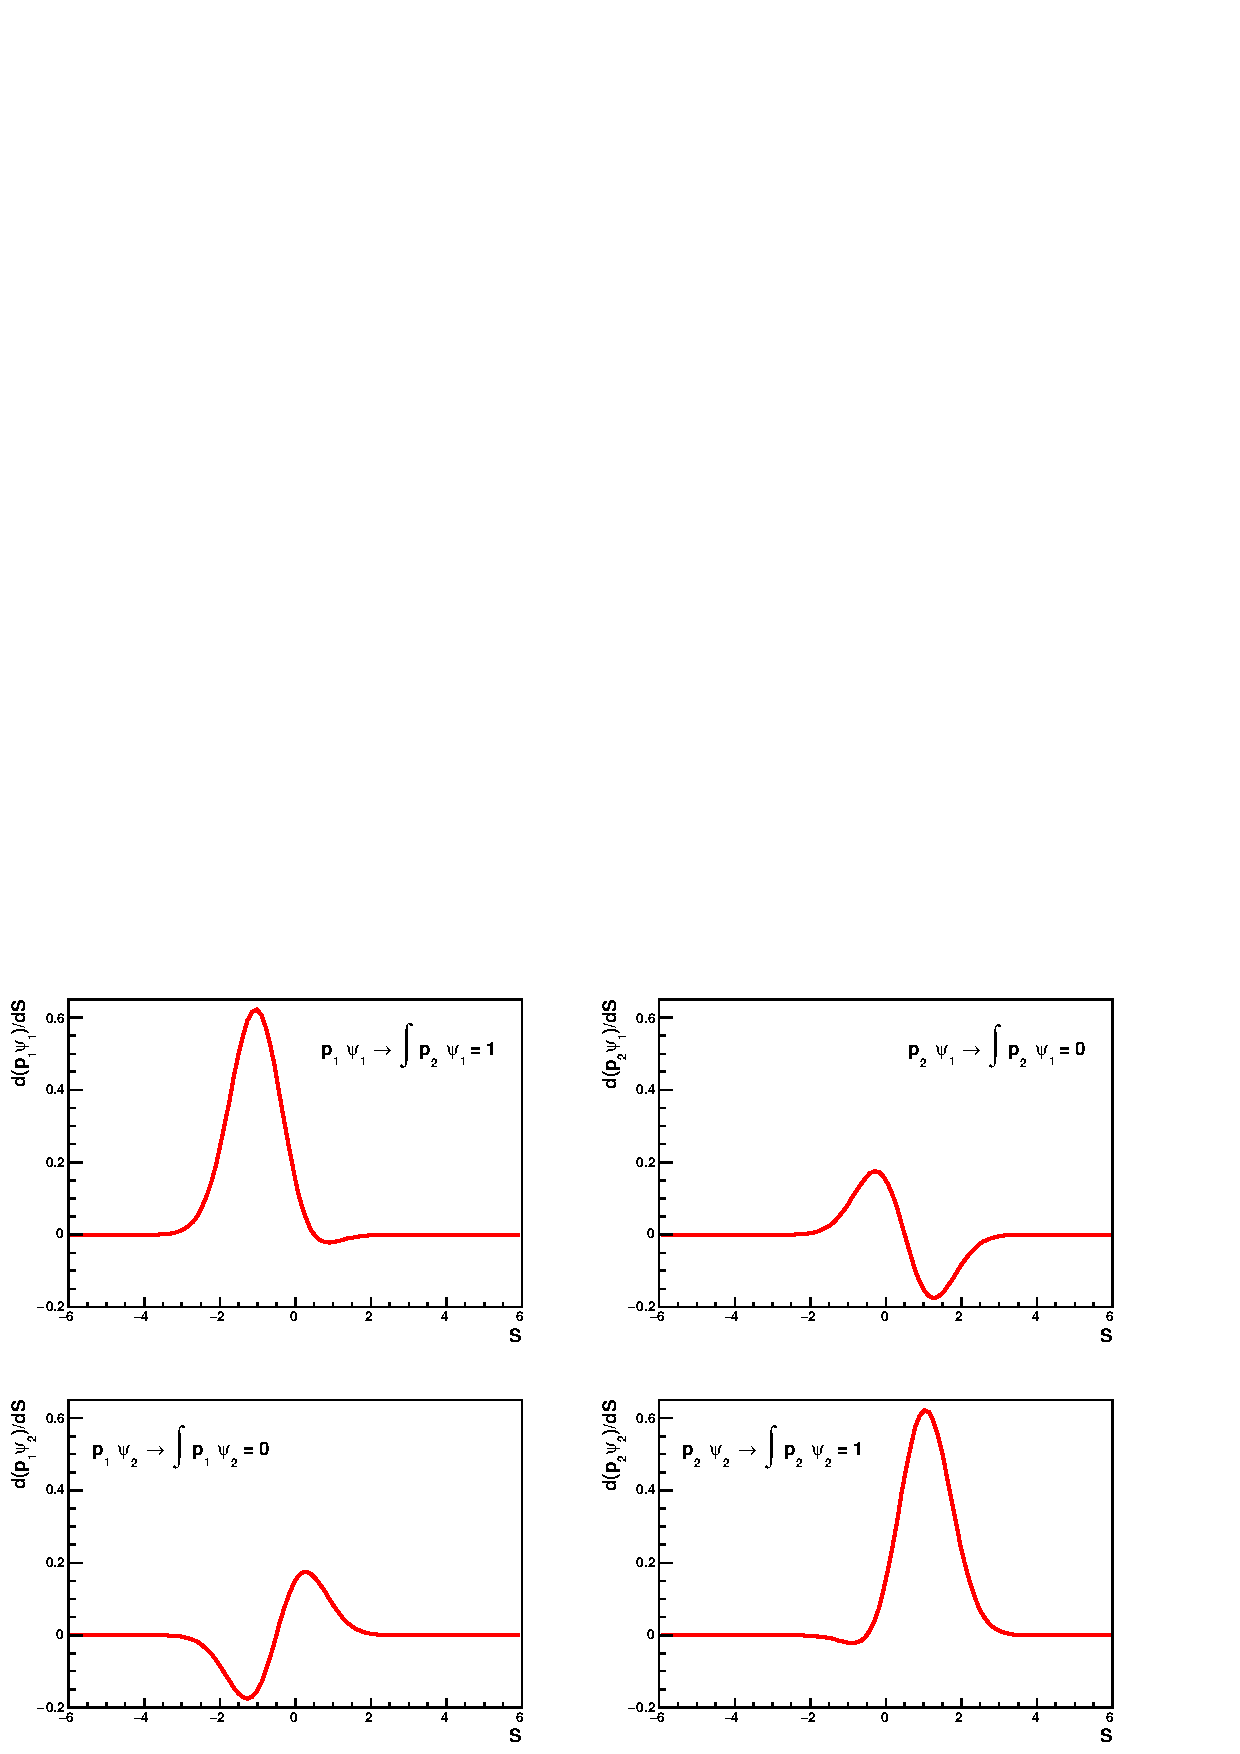
\includegraphics[width=0.7\textwidth]{../png/figSPgaus.png}
\caption{Scalar product functions for the two Gaussian responses case ($\Delta_{12} = 2$).}
\label{fig:SPGaus2}
\end{figure}


\begin{figure}[!htb]
\centering
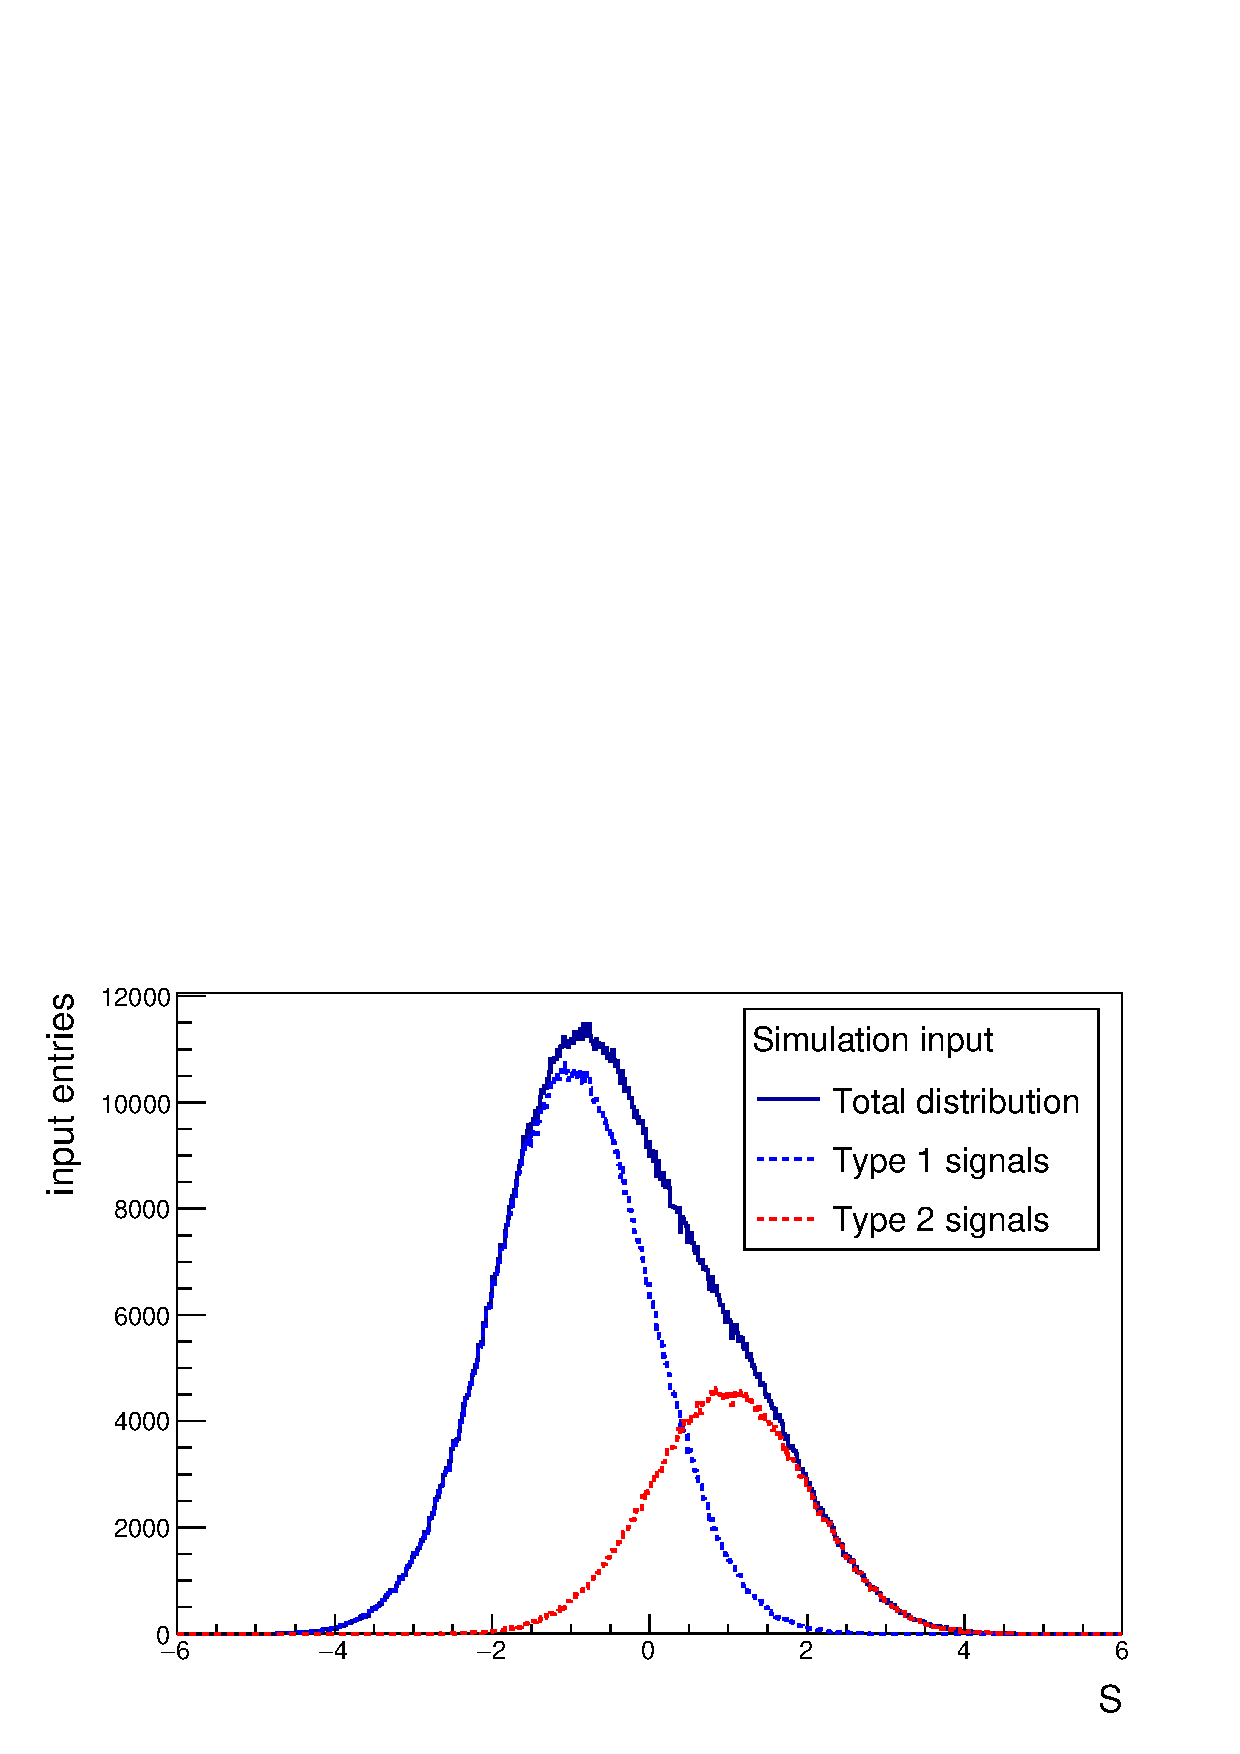
\includegraphics[width=0.7\textwidth]{../png/figInput.png}
\caption{Inputs of the simulation (type 1: 70\%, type 2: 30\%).}
\label{fig:InputGaus2}
\end{figure}

\begin{figure}[!htb]
\centering
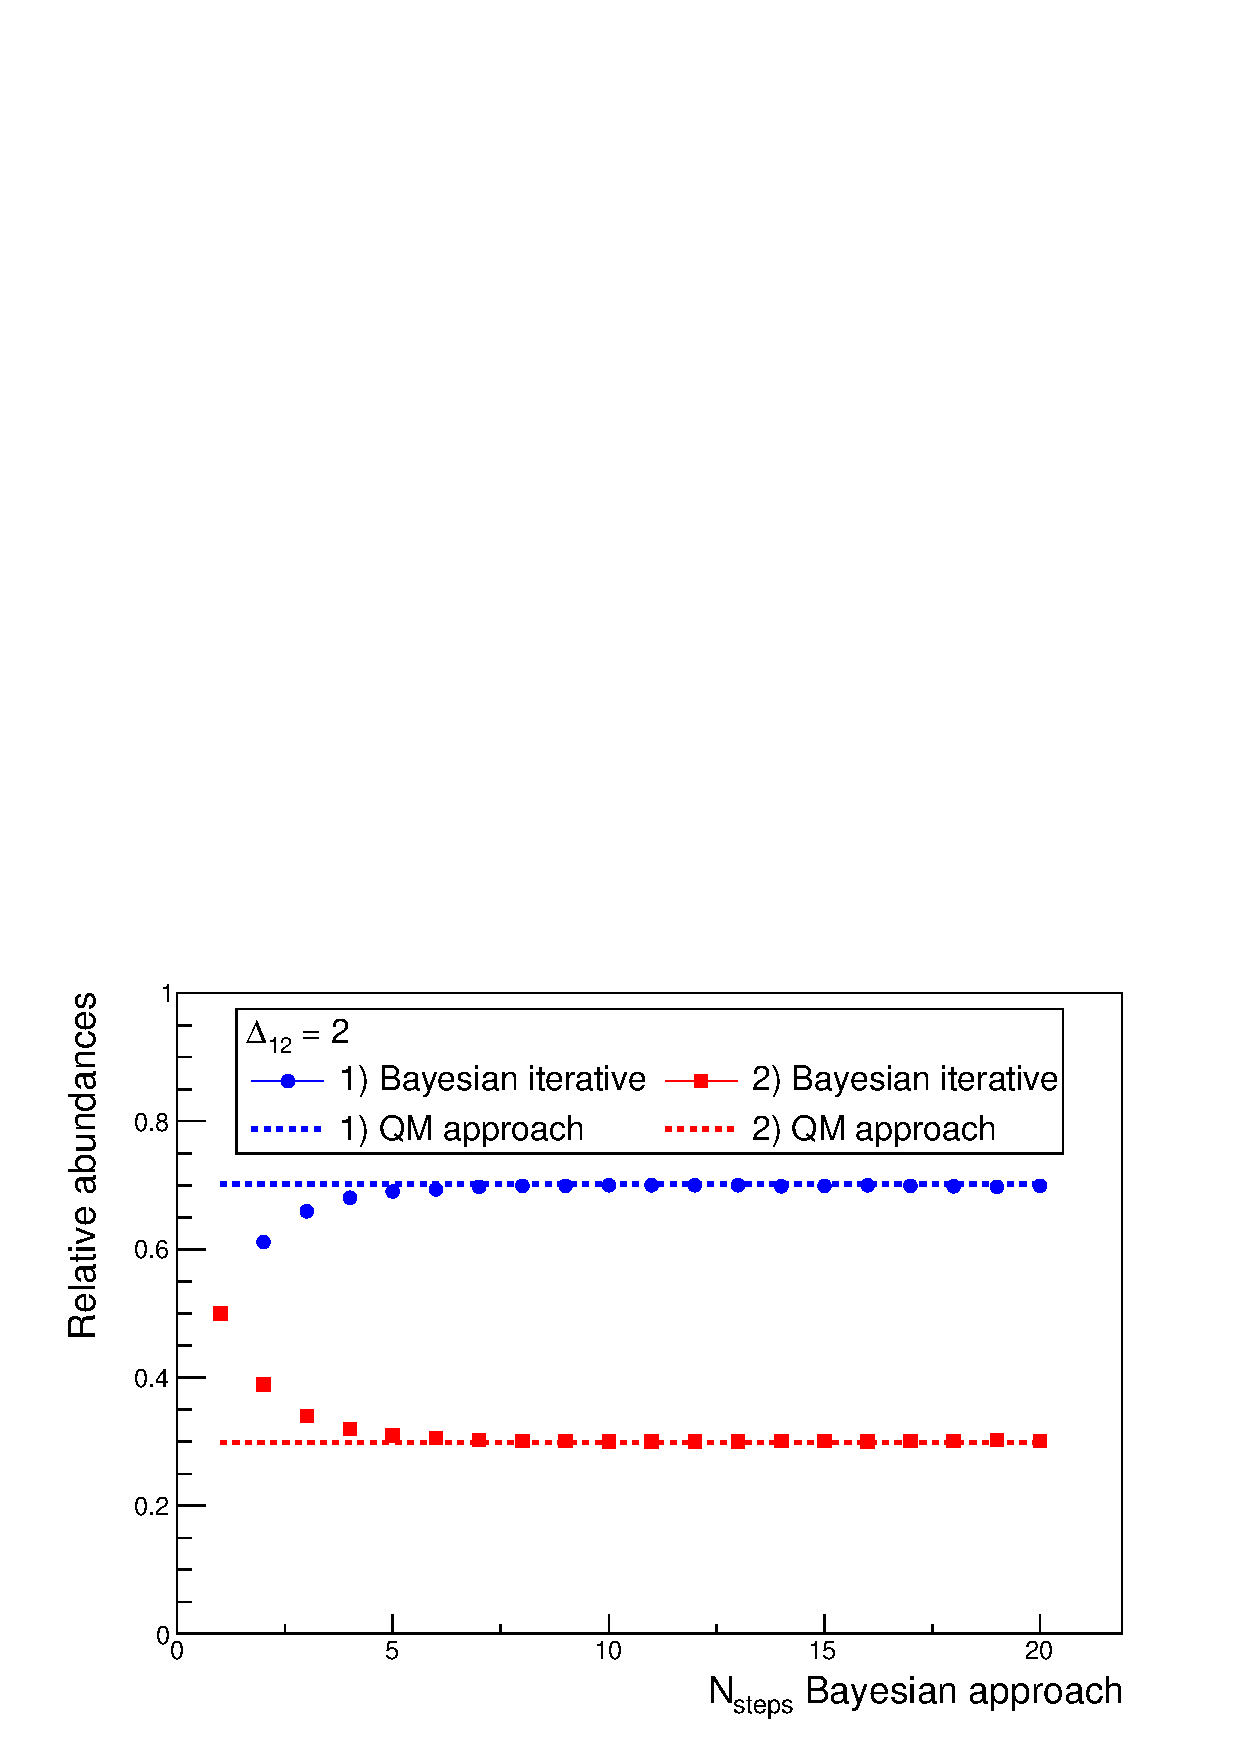
\includegraphics[width=0.45\textwidth]{../png/figIterativeDelta2.png}
\includegraphics[width=0.45\textwidth]{../png/figIterativeDelta1.png}
\caption{Comparison of the two approaches: results for $\Delta_{12} = 2$ and
  $\Delta_{12} = 1$ cases.}
\label{fig:IterGaus2}
\end{figure}

\subsection{Multi-variables case}

\subsection{Correlations of event pair}

